\chapter[Análisis Financiero]{Análisis Financiero}

\section{Análisis financiero del hardware}
En el análisis financiero del proyecto se analizaron los gastos teniendo en cuenta  recursos materiales y humanos utilizados. Para el calcular el proceso de esfuerzo humano se realizó un promedio del salario en base a un desarrollador de software en Paraguay, como el proyecto está hecho con lenguajes de programación web para el software y lenguaje C para el hardware se vio que los Desarrolladores web y multimedios ganan normalmente un salario neto mensual aproximado de entre Gs. 3.000.000 y Gs. 6.000.000 al empezar en el puesto de trabajo, esto según las referencias obtenidas de la página tusalario.org, \cite{tusalario}, así haciendo un promedio y suponiendo 20 días de trabajo al mes con 8 horas diarias, el costo por horas de trabajo es de 30 000Gs por hora aproximadamente. Se aborda este salario para el trabajo en backend, frontend, desarrollo de hardware y su programación. 


En la  \textbf{tabla \ref{tabla:hw}} observamos el costo de los componentes utilizados para el hardware, además de las herramientas utilizadas para su elaboración. 



%%%%%%%%%%%%%%%%%%%%% tabla %%%%%%%%%%%%%%%%%%%%%%%%%%%%%%%%
\begin{table}[H]
\begin{center}
\begin{tabular}{|c|l|l|r|r|}
\hline
\textbf{Cant} & \textbf{Componente} & \textbf{Valor} &\textbf{Unidad}&\textbf{Importe}  \\ \hline

2    & Capacitores      & 10uF        & 250            & 500   \\ \hline
2    & Capacitores      & 0,1uF       & 250            & 500   \\ \hline
2    & Capacitores      & 15pf        & 1000           & 2000  \\ \hline
1    & Resistor         & 330 ohm     & 250            & 250   \\ \hline
1    & Resistor         & 100k        & 250            & 250   \\ \hline
1    & Microcontrolador &PIC18F4580   & 85000          & 85000 \\ \hline
1    & Regulador        & 7805        & 15000          & 15000 \\ \hline
2    & Diodo            & 1N4148      & 1000           & 2000  \\ \hline
1    & Diodo Led        & Rojo        & 1000           & 1000  \\ \hline
1    & Botón            & 4 pines    & 3500           & 3500  \\ \hline
1    & Conector        & DB9    & 5000           & 5000  \\ \hline
1    & Espadines       & 5 pines   & 3500           & 3500  \\ \hline
2    & Módulo          & SHIELD & 55000          & 110000 \\ \hline
2    & Módulo          & XBEE        & 250000         & 500000 \\ \hline
2    & Espadines       & 20 pines  & 3500           & 7000    \\ \hline
1    & Módulo          & MCP2551     & 30000          & 30000  \\ \hline
1    & Cristal         & 16Mhz     & 5000           & 5000   \\ \hline
1    & Placa de Cobre  & 1 Capa      & 13000          & 13000   \\ \hline
1    & Conector OBD II  & OBD II     & 50000          & 50000   \\ \hline
1    & Impresora 3D         & Caja 3D       & 100000         & 100000 \\ \hline
1    & Fresadora CNC    & CNC        & 100000         & 100000 \\ \hline
     &                  &            & \textbf{Total} & \textbf{1 033 500}  \\ \hline

\end{tabular}
\caption{Costo de los componentes y herramientas usadas en el hardware.}
\label{tabla:hw}
\end{center}
\end{table}

Para la programación  y diseño organizaremos el trabajo en diseño del hardware, programación del hardware, Programación del Software frontend y backend, cada uno con un costo de 30 000Gs. la hora, resultando lo visto en la \textbf{tabla \ref{tabla:software}}. 

%%%%%%%%%%%%%%%%%%%%% tabla %%%%%%%%%%%%%%%%%%%%%%%%%%%%%%%%
\begin{table}[H]
\begin{center}
\begin{tabular}{|l|r|r|r|}
\hline
\textbf{Trabajo Realizado} & \textbf{Horas}&\textbf{Salario por hora Gs.} & \textbf{Importe Gs.} \\ \hline

 Placa Electrónica & 320 & 30 000  & 6 400 000     \\ \hline
 Software CAN      & 640 & 30 000  & 12 800 000     \\ \hline
 Diseño de Usuario & 640 & 30 000  & 12 800 000     \\ \hline
 Programación del Servidor & 640 & 30 000 & 12 800 000 \\ \hline 
  &  & Total Costos & 44 800 000 \\ \hline 

\end{tabular}
\caption{Tabla Costos de mano de obra.}
\label{tabla:software}
\end{center}
\end{table}
%%%%%%%%%%%%%%%%%%%%%%%%%%%%%%%%%%%%%%%%%%%%%%%%%%%%%%%%%%%%%%%%%%%%



En la \textbf{tabla \ref{tabla:licencias}} observamos el costo de las licencias de Proteus  \cite{licenp}, y el compilador PIC CCS \cite{pic_ccs}.
%%%%%%%%%%%%%%%%%%%%% tabla %%%%%%%%%%%%%%%%%%%%%%%%%%%%%%%%
%%%% \textbf{tabla \ref{tabla:hw}} 
\begin{table}[H]
\begin{center}
\begin{tabular}{|l|l|l|}
\hline
\textbf{Herramienta} & \textbf{Licencia} & \textbf{Costo}  \\ \hline
Proteus Starter Kit  & Básica & 1 600 000  \\ \hline
Compilador PIC CCS   & PIC18  & 1 400 000  \\ \hline

\textbf{Total} &  &   3 000 000     \\ \hline
\end{tabular}
\caption{Tabla Costos de Licencias.}
\label{tabla:licencias}
\end{center}
\end{table}
%%%%%%%%%%%%%%%%%%%%%%%%%%%%%%%%%%%%%%%%%%%%%%%%%%%%%%%%%%%%%%%%


En la \textbf{tabla \ref{tabla:total}} presentamos el costo total del proyecto teniendo en cuenta los resultados de las tablas anteriores: 

%%%%%%%%%%%%%%%%%%%%% tabla %%%%%%%%%%%%%%%%%%%%%%%%%%%%%%%%
%%%% \textbf{tabla \ref{tabla:hw}} 
\begin{table}[H]
\begin{center}
\begin{tabular}{|l|l|l}
\hline
\textbf{Referencia} & \textbf{Costos}  \\ \hline

Costos Hardware  & 1 033 500     \\ \hline
Costos Software  & 44 800 000     \\ \hline
Costos Licencias & 3 000 000     \\ \hline

\textbf{Total} & 48 833 500    \\ \hline
\end{tabular}
\caption{Tabla costos totales.}
\label{tabla:total}
\end{center}
\end{table}
%%%%%%%%%%%%%%%%%%%%%%%%%%%%%%%%%%%%%%%%%%%%%%%%%%%%%%%%%%%%%%%%


\section{Mejoras Futuras del hardware y del sistema}
Con más tiempo de desarrollo y con un presupuesto considerable se podría diseñar mejoras al prototipo del sistema,como reducir el tamaño físico del dispositivo y complementarlo con una computador Raspberry Pi con la posibilidad de convertirse en un servidor de datos para otros puntos de acceso, por ejemplo: que una vez conectado el módulo CAN al vehículo, otros dispositivos como computadoras y celulares puedan acceder a los datos leídos mediante una red o por sistemas como wifi o bluetooth, al mismo tiempo que el propio dispositivo despliega los datos en una propia pantalla, de esta manera se tendría versatilidad en su uso. 

En la \textbf{ Figura \ref{fig_raspberri_c4}} se observa la propuesta con tres bloques de funcionamiento, en el \textbf{bloque 1} el hardware CAN se conectaría al vehículo y se encargaría de las lecturas del sistema, así mediante bluetooth se conectaría al \textbf{bloque 2} con la Raspberri Pi, el cual sería responsable de la visualización de los datos. Hasta aquí se tendría un sistema CAN OBD II completo, pero adicionalmente en el \textbf{bloque 3} se muestra como el software del proyecto está preparado para conectarse a una red de internet para que otros dispositivos tengan acceso a los datos del vehículo, el módulo Wifi o el puerto Ethernet ya está incorporado en la Raspberry Pi para esta funcionalidad, siendo solo necesario obtener  de las compañías proveedoras de internet los permisos correspondientes. 

%%%%%%%%%%%%%%%%%%%%%%%%%%%%%%%%%%%%%%%%%%%%%%%%%%%%%%%%%%
\begin{figure}[H]
	\centering
		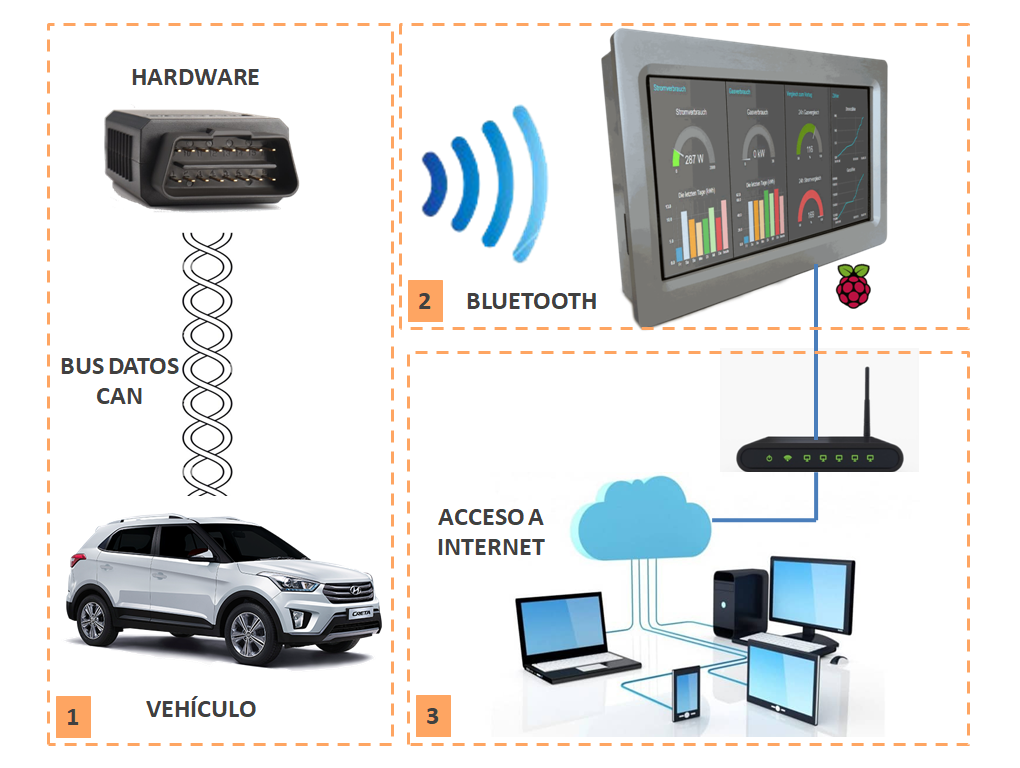
\includegraphics[width=0.9\textwidth]{./Cap00imagen/fig_raspberri_f.png}
	\caption[Sistema CAN con raspberry Pi.]{Sistema CAN con raspberry Pi.\textbf{ Fuente:}  Elaboración Propia.}
	\label{fig_raspberri_c4} % Etiqueta para la referencia.
\end{figure}

% CITAR IMAGEN
%%%%%%%%%%%%%%%%%%%%%%%%%%%%%%%%%%%%%%%%%%%%%%%%%%%%%%%%%%

Para reducir el tamaño físico de hardware CAN se presupuesta usar componentes electrónicos de montajes superficiales y agregar un módulo bluetooth para la conección con la computadora Raspberry PI, el presupuesto aproximado de la fabricación completa se logró obtener con la ayuda de la empresa PCBway \cite{pcbway}, ya que posee unos pasos a seguir para el calculo de presupuesto para la fabricación completa de un circuito en PCB con los componentes incluidos. En la \textbf{tabla \ref{tabla:raspberri}} se muestran el presupuesto del hardware para este nuevo sistema.
%%%%%%%%%%%%%%%%%%%%% tabla %%%%%%%%%%%%%%%%%%%%%%%%%%%%%%%%
\begin{table}[H]
\begin{center}
\begin{tabular}{|l|l|r|}
\hline
\textbf{Elementos} & \textbf{Comentario} & \textbf{Costo}  \\ \hline


Hardware CAN    & PCB Fabricado    & 918 000 \\ \hline
Conector        & OBD II - J1939     & 50 000 \\ \hline
Módulo          & Bluetooth          & 60 000 \\ \hline
Computadora     & Raspberrry PI 4    & 600 000 \\ \hline
Pantalla TFT    & 4 pulgadas         & 300 000 \\ \hline
Protector       & Caja 3D            & 150 000\\ \hline
\textbf{Total Costos}&  &2 078 000 \\ \hline



\end{tabular}
\caption{Costo de los elementos para una propuesta mejorada del sistema CAN.}
\label{tabla:raspberri}
\end{center}
\end{table}





